\documentclass{article}
\usepackage[utf8]{inputenc}
\usepackage[russian]{babel}
\usepackage{graphicx}
\usepackage{amsmath}
\usepackage{breqn}
\usepackage{wrapfig}
\usepackage{float}
\usepackage{multirow}
\usepackage{caption}
\usepackage{subcaption}

\graphicspath{ {./data/images} }
\author{Александр Романов Б01-107}
\date{}
\title{8.1 Определение постоянных Стефана-Больцмана и Планка из анализа теплового излучения накалённого тела}

\begin{document}
\maketitle
\section{Введение}
\subsection{Краткое описание}
При помощи модели абсолютно чёрного тела проводятся измерения температуры оптическим пирометром с ичезающей
нитью и термопарой, исследуется излучение накалённых тел с различной испускательной способностью, 
определяются постоянные Планка и Стефана-Больцмана.
\subsection{Теоретическая справка}
Если бы нить излучала как АЧТ, то баланс потребляемой и излучаемой энергии был бы:
\[ W = \sigma S\left(T^4 - T0^4\right) \]
где \(W\) - потребляемая нитью электрическая мощность, \(S\) - площадь излучающей поверхности нити,
\(T\) - температура нити, \(T_0\) - температура окружающей среды.

Если предположить, что нить излучает как серое тело, то выражение можно записать в виде:
\[ W = \varepsilon_T S\sigma T^4\]

\subsection{Экспериментальная установка}
\begin{figure}[H]
	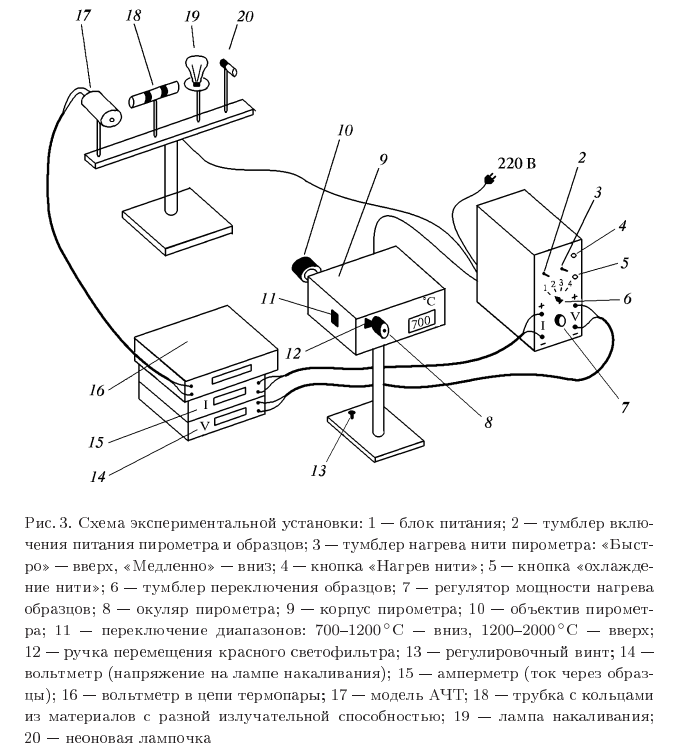
\includegraphics[width=\textwidth]{scheme.png}
\end{figure}
\section{Работа}
\subsection{Изучение работы оптического пирометра}
В этой части работы мы измерим температуру модели АЧТ с помощью пирометра и сравним её с температурой,
полученной по термопаре.

Включив пирометр будем методом последовательных приближений изменять его температуру так, чтобы определить
момент визуального исчезновения нити на фоне АЧТ. Получим значение \(T = 1190\pm 20^\circ C\). При этом
показания термопары: \(U_p = 47.25\; mV\). Учитывая постоянную термопары (\( 41\; \mu V/^\circ C \)) получим
значение температуры:
\[T_p = 41 \cdot U_p = 1173\pm + 21^\circ C = 1173 \pm ^\circ C\]
Значение температуры, полученное при помощи пирометра, совпадает с температурой термопары в пределах
погрешности.

\subsection{Проверка закона Стефана-Больцмана}
Направим пирометр на нить лампы накаливания и включим её. Постепенно увеличивая накал нити лампы, начиная
со слабого тёмно-красного накала (\(\simeq 900^\circ C\)) вплоть до \(1900^\circ C\). Помимо температуры
необходимо записывать также величину тока и напряжения на нити лампы.

\begin{table}[H]
	\begin{tabular}{|c|c|c|c|c|c|c|c|c|c|c|c|}
		\hline
		\(T, ^\circ C\) & 900   & 1000  & 1100  & 1200  & 1300 & 1400 & 1500 & 1600 & 1700 & 1800 & 1900 \\\hline
		\(I, A\)				& 0.625 & 0.702 & 0.806 & 0.902 & 1    & 1.08 & 1.15 & 1.23 & 1.31 & 1.4  & 1.5  \\\hline
		\(U, V\)				& 15.8  & 20.87 & 29    & 37    & 46.4 & 54   & 60.3 & 69.1 & 78   & 88.3 & 100  \\\hline
		\(P = IV, J\)      & 9.88  & 14.65 & 23.37 & 33.37 & 46.40 & 58.32 & 69.34 & 84.99 & 102.18 & 123.62 & 150.00 \\\hline
	\end{tabular}
\end{table}

Построим график \(P = f(T)\):

\begin{figure}[H]
	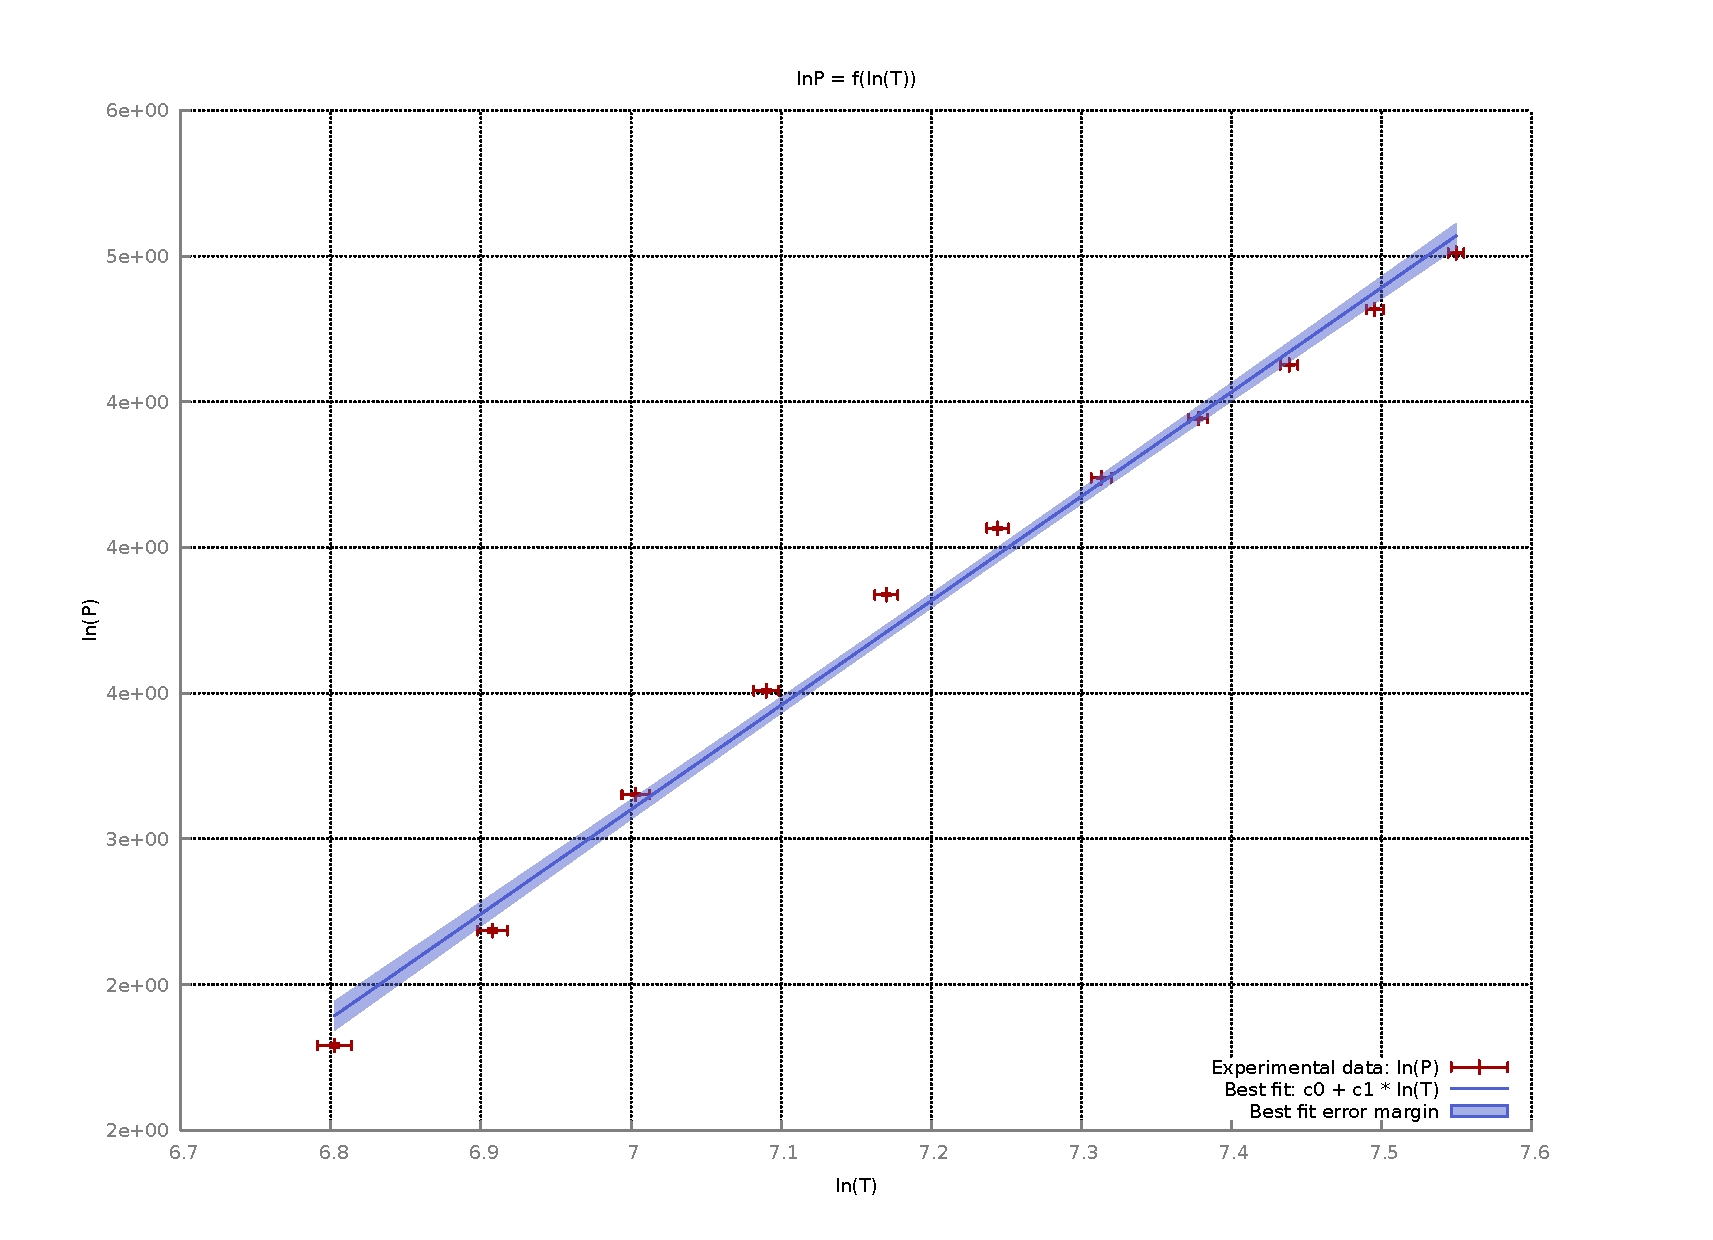
\includegraphics[width=\textwidth]{plot.pdf}
\end{figure}

Получили зависимость вида \( y = k\cdot x + b \):
\[ k = 3.58 \pm 0.10 \]
\[ b = -21.97 \pm 0,7 \]


Полученное значение углового коэффициента (\( k = 3.58 \pm 0.10 \)) достаточно точно совпадает со
значением 4, следующем из закона Стефана-Больцмана:
\[ P = \sigma \varepsilon_T S T^4  \]

Найдём значение постоянной Стефана-Больцмана по формуле:
\[ \sigma = \frac{P}{\varepsilon_T}{ST^4} = 3.2\cdot 10^{-4}\; \frac{Wt}{m^2 K^4} \]

Полученное значение на несколько порядков отличается от табличного: \( \sigma = 5.66\cdot 10^{-8}\; \frac{Wt}{m^2K^4} \)
\subsection{Измерение яркостной температуры накалённых тел}
Нагре кольца и керамическую трубку до одинаковых температур убедимся что разные температуры имеют различную
яркостную температуру при одинаковой термодинамической температуре.
\subsection {Измерение яркостной температуры неоновой лампочки}

Направим пирометр на неоновую лампочку. Измерим при помощи него яркостную температуру неоновой лампочки.
\[ T = 914\; K \]
Однако дотронувшись до лампочки рукой убедимся что её температура даже не близка к \(900\; K\).
\section{Выводы}
В ходе работы:
\begin{enumerate}
\item Был проверен закон Стефана-Больцмана и получен коэффициент степени \(T\), который достаточно точно совпадает с теоретическим:
	\[ 3.58 \pm 0.1 VS 4 \]
\item Было найдено значение постоянной Стефана-Больцмана. Однако значение отличается от табличного на несколько порядков:
	\[ 3.2\cdot 10^{-4} VS 5.66\cdot 10^{-8} \frac{Wt}{m^2K^4} \]
\item Было проверено, что разные материалы имеют разную яркостную температуру при равной термодинамической.
	Также объекты с высокой яркостной температурой могут иметь маленькую термодинамическую.
\end{enumerate}
\end{document}
